%%%%%%%%%%%%%%%%%%%%%%%%%%%%%%%%%%%%

\section{Small sample inference for a proportion}

%%%%%%%%%%%%%%%%%%%%%%%%%%%%%%%%%%%%

\subsection{Paul the octopus}

%%%%%%%%%%%%%%%%%%%%%%%%%%%%%%%%%%%%

\begin{frame}
\frametitle{Famous predictors}

\twocol{0.5}{0.5}{
Before this guy...
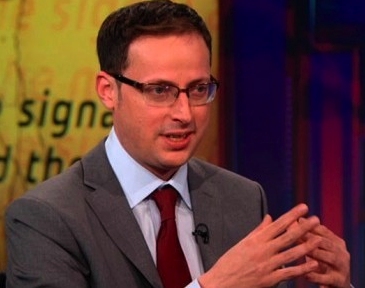
\includegraphics[width=\textwidth]{6-5_small_single_prop/figures/paul/nate}
}
{
\pause
There was this guy...
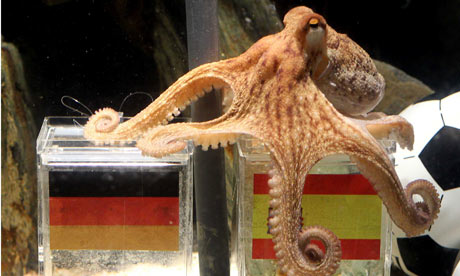
\includegraphics[width=\textwidth]{6-5_small_single_prop/figures/paul/paul}
}

\end{frame}

%%%%%%%%%%%%%%%%%%%%%%%%%%%%%%%%%%

\begin{frame}
\frametitle{Paul the Octopus - psychic?}

\begin{itemize}

\item Paul the Octopus predicted 8 World Cup games, and predicted them all correctly  

\pause

\item Does this provide convincing evidence that Paul actually has psychic powers?

\pause

\item How unusual would this be if he was just randomly guessing (with a 50\% chance of 
guessing correctly)?

\pause

\item Hypotheses:
\begin{itemize}
\item[$H_0:$] $p = 0.5$
\item[$H_A:$] $p > 0.5$
\end{itemize}

\end{itemize}

\end{frame}

%%%%%%%%%%%%%%%%%%%%%%%%%%%%%%%%%%

\begin{frame}
\frametitle{Conditions}

\begin{enumerate}

\item \hl{Independence:} We can assume that each guess is independent of another.

\pause

\item \hl{Sample size:} The number of expected successes is \orange{smaller than 10}.
\[ 8 \times 0.5 = 4 \]

\end{enumerate}

\pause

\vspace{1cm}

\dq{So what do we do?}

\pause

Since the sample size isn't large enough to use CLT based methods, we use a simulation method instead.

\end{frame}

%%%%%%%%%%%%%%%%%%%%%%%%%%%%%%%%%%

\begin{frame}
\frametitle{}

\pq{Which of the following methods is best way to calculate the p-value of the hypothesis test evaluating if Paul the Octopus' predictions are unusually higher than random guessing?}

\begin{enumerate}[(a)]
\item Flip a coin 8 times, record the proportion of times where all 8 tosses were heads. Repeat this many times, and calculate the proportion of simulations where all 8 tosses were heads.
\item Roll a die 8 times, record the proportion of times where all 8 rolls were 6s. Repeat this many times, and calculate the proportion of simulations where all 8 rolls were 6s.
\item Flip a coin 10,000 times, record the proportion of heads. Repeat this many times, and calculate the proportion of simulations where more than 50\% of tosses are heads.
\item Flip a coin 10,000 times, calculate the proportion of heads.
\end{enumerate}

\end{frame}

%%%%%%%%%%%%%%%%%%%%%%%%%%%%%%%%%%%

\begin{frame}
\frametitle{Simulate}

\pq{Flip a coin 8 times. Did you get all heads?}

\begin{enumerate}[(a)]
\item Yes
\item No
\end{enumerate}

\end{frame}

%%%%%%%%%%%%%%%%%%%%%%%%%%%%%%%%%%

\begin{frame}[fragile]
\frametitle{}

{\tiny
\begin{Verbatim}[frame=single, formatcom=\color{blue}]
source("http://www.openintro.org/stat/slides/inference.R")
paul = factor(c(rep("yes", 8), rep("no", 0)), levels = c("yes","no"))
inference(paul, est = "proportion", type = "ht", method = "simulation",
          success = "yes", null = 0.5, alternative = "greater", seed = 290)
\end{Verbatim}
}

\pause

{\tiny
\begin{Verbatim}[frame=single, formatcom=\color{gray}]
Single proportion -- success: yes 
Summary statistics: p_hat = 1 ;  n = 8 
H0: p = 0.5 
HA: p > 0.5 
p-value =  0.0037
\end{Verbatim}
}

\centering
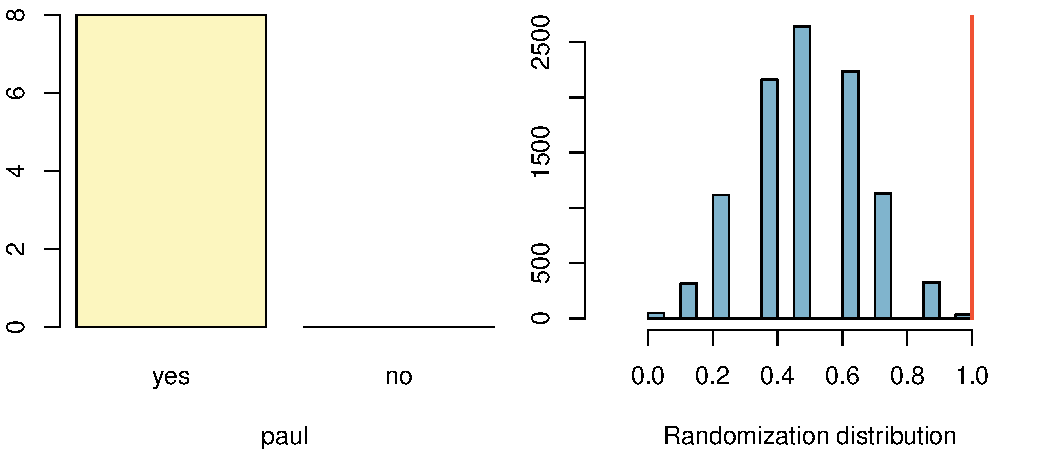
\includegraphics[width=0.8\textwidth,height=0.4\textheight]{6-5_small_single_prop/figures/paul/paul_HT}

\end{frame}

%%%%%%%%%%%%%%%%%%%%%%%%%%%%%%%%%%%

\begin{frame}
\frametitle{Conclusions}

\pq{Which of the following is \underline{false}?}

\begin{enumerate}[(a)]

\item If in fact Paul was randomly guessing, the probability that he would get the result of all 8 games correct is 0.0037.

\item Reject $H_0$, the data provide convincing evidence that Paul did better than randomly guessing.

\item We may have made a Type I error.

\solnMult{The probability that Paul is psychic is 0.0037.}

\end{enumerate}

\end{frame}

%%%%%%%%%%%%%%%%%%%%%%%%%%%%%%%%%%%%

\subsection{Back of the hand}

%%%%%%%%%%%%%%%%%%%%%%%%%%%%%%%%%%%

\begin{frame}
\frametitle{Back of the hand}

\dq{There is a saying ``know something like the back of your hand". Describe an experiment to test if people really do know the backs of their hands.}

\pause

\begin{center}
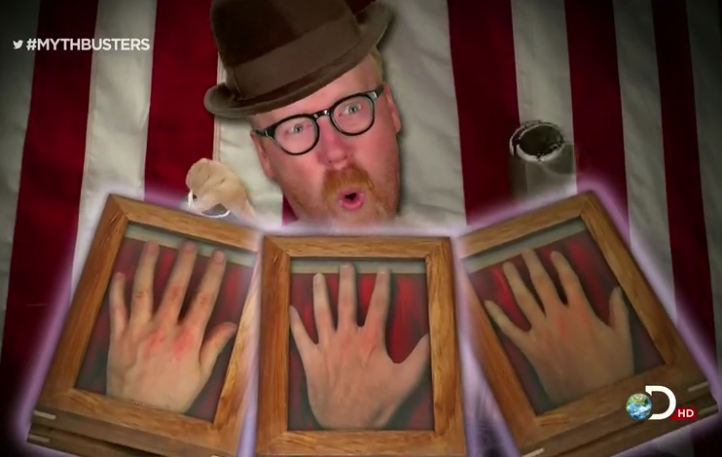
\includegraphics[width=0.6\textwidth]{6-5_small_single_prop/figures/hand/mythbusters}
\end{center}

In the MythBusters episode, 11 out of 12 people guesses the backs of their hands correctly.

\end{frame}

%%%%%%%%%%%%%%%%%%%%%%%%%%%%%%%%%%%%

\begin{frame}
\frametitle{Hypotheses}

\dq{What are the hypotheses for evaluating if people are capable of recognizing the back of their hand at a rate that is better than random guessing. Remember, in the MythBusters experiment, there were 10 pictures to choose from, and only 1 was correct.}

\begin{itemize}
\item[$H_0:$] $p = 0.10$ (random guessing)
\item[$H_A:$] $p > 0.10$ (better than random guessing)
\end{itemize}

\end{frame}

%%%%%%%%%%%%%%%%%%%%%%%%%%%%%%%%%%%

\begin{frame}
\frametitle{Conditions}

\begin{enumerate}

\item \hl{Independence:} We can assume that each person guessing is independent of another.

\item \hl{Sample size:} The number of expected successes is \orange{smaller than 10}.
\[ 12 \times 0.1 = 1.2 \]

\end{enumerate}

\dq{So what do we do?}

Since the sample size isn't large enough to use CLT based methods, we use a simulation method instead.

\end{frame}

%%%%%%%%%%%%%%%%%%%%%%%%%%%%%%%%%%%

\subsection{Randomization HT for a proportion}

%%%%%%%%%%%%%%%%%%%%%%%%%%%%%%%%%%%%

\begin{frame}
\frametitle{Simulation scheme}

\dq{Describe how you test if results of this experiment to determine if people are capable of recognizing the back of their hand at a rate that is better than random guessing.}
\vspace{-0.5cm}
\[ H_0: p = 0.10 \qquad H_A: p > 0.10 \qquad \hat{p} = 11 / 12 = 0.9167 \]

\begin{enumerate}

\item Use a 10-sided fair die to represent the sampling space, and call 1 a success (guessing correctly), and all other outcomes failures (guessing incorrectly).

\item Roll the die 12 times (representing 12 people in the experiment), count the number of 1s, and calculate the proportion of correct guesses in one simulation of 12 rolls.

\item Repeat step (2) many times, each time recording the proportion of successes in a series of 12 rolls of the die.

\item Create a dot plot of the simulated proportions from step (3) and count the number of simulations where the proportion was at least as high as 0.9167 (the observed proportion).

\end{enumerate}

\end{frame}

%%%%%%%%%%%%%%%%%%%%%%%%%%%%%%%%%%%

\begin{frame}
\frametitle{Simulation results}

\begin{itemize}

\item In the next slide you can see the results of a hypothesis test (using only 100 simulations to keep things simple).

\item Each dot represents a simulation proportion of success. There were 25-30 simulations where the success rate ($\hat{p}$) was 10\%, 40-45 simulations where the success rate was slightly less than 10\%, about 20 simulations where the success rate was slightly less than 20\% and 1 simulation where the success rate was more than 30\%.

\item There are no simulations where the success rate is as high as the observed success rate of 91.67\%.

\item Therefore we conclude that the observed result is near impossible to have happened by chance (p-value = 0).

\item And hence that these data suggest that people are capable of recognizing the back of their hand at a rate that is better than random guessing. 

\end{itemize}

\end{frame}

%%%%%%%%%%%%%%%%%%%%%%%%%%%%%%%%%%%%

\begin{frame}[fragile]
\frametitle{}

{\tiny
\begin{Verbatim}[frame=single, formatcom=\color{blue}]
back = as.factor(c(rep("correct", 11), rep("wrong", 1))) 
inference(back, est = "proportion", type = "ht", method = "simulation",
	success = "correct", null = 0.1, alternative = "greater", seed = 654, nsim = 100)
\end{Verbatim}
}

\pause

{\tiny
\begin{Verbatim}[frame=single, formatcom=\color{gray}]
Single proportion -- success: correct 
Summary statistics: p_hat = 0.9167 ;  n = 12 
H0: p = 0.1 
HA: p > 0.1 
p-value =  0 
\end{Verbatim}
}

\centering
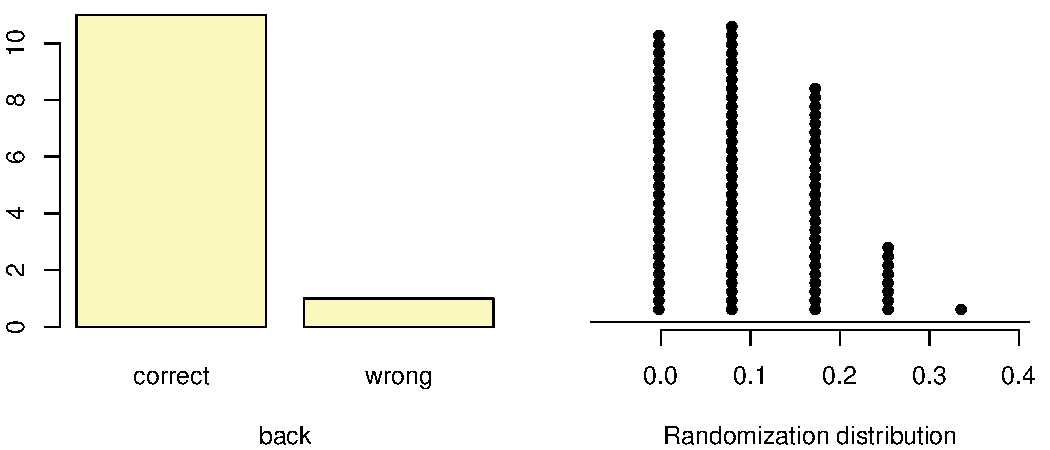
\includegraphics[width=0.8\textwidth,height=0.4\textheight]{6-5_small_single_prop/figures/hand/back_HT}

\end{frame}

%%%%%%%%%%%%%%%%%%%%%%%%%%%%%%%%%%%